\subsection{Modelling}
หลังจากที่เราได้ออกแบบและโมเดลหุ่นยนต์ของเราขึ้นมาที่ใช้ CAD tools ต่างๆ เช่น AutoCAD, SolidWorks, Blender
หรืออื่นๆ ก็เพื่อที่จะนำมาใช้ในการทำ Simulation การที่เราทำ Simulation นั้นก็จะสามารถมองเห็นหุ่นยนต์
และเห็นการทำงานของหุ่นยนต์เราก่อนที่เราจะสร้างมันขึ้นมาจริงๆ หุ่นยนต์จำลองที่เราสร้างขึ้นมานั้นควรที่จะมีลักษณะให้ใกล้เคียงกับของจริงมากที่สุด
ไม่ว่าจะเป็นรูปร่าง รูปทรง น้ำหนักต่างๆ 

\subsubsection{ROS packages for robot modelling}
ROS นั้นได้ให้เครื่องมือที่ช่วยให้เราสามารถสร้าง 3D robot models ได้
ใน ROS มี meta package ที่ชื่อว่า robot\_model ซึ่งข้างในมี package ต่างๆที่ใช้สำหรับสร้าง 3D robot models
        
\paragraph*{urdf}
เป็น 1 ในหลายๆ package ที่อยู่ใน robot\_model, urdf เป็น xml ไฟล์ที่เอาไว้ใช้บอกลักษณะของหุ่นยนต์ ย่อมาจาก Unified Robot Description Format(URDF)
เราสามารถระบุ robot model, sensors และ working environment โดยใช้ URDF การบอกนั้นจะสามารถบอกเป็นเหมือน tree structure ของ link ต่างๆในตัวหุ่นยนต์ สามารถบอก rigid link เชื่อมต่อกันผ่าน joints แต่ถ้าเป็น flexible link จะไม่สามารถบอกได้โดยใช้ urdf

\subparagraph*{joint\_state\_publisher}
เครื่องมือนี้มีประโยชน์มากในการ model robot URDF เพราะมันสามารถหา joints ทุก joint ที่ไม่ใช่ fixed joints มาแสดงเป็น GUI sliders ทำให้เราสามารถเลื่อนๆหมุนๆไปมาได้ อีกทั้งยังสามารถใช้งานร่วมกับ visualize RViz

\subparagraph*{robot\_state\_publisher}
เป็นเครื่องมือที่ใช้ในการ publish 3d pose ของ link ต่างๆใน urdf การ publish นั้นจะใช้ ROS tf(transform) ROStf คือการหาความสัมพันธ์ระหว่าง frame ของหุ่นยนต์

\subparagraph*{xacro}
ย่อมาจาก XML Macros หรือเราสามารถเรียกอีกอย่างว่า URDF plus add-ons. ซึ่งการทำงานเหมือนกับ urdf แต่ทำให้ไฟล์ urdf สั้นกว่า อ่านง่ายกว่า และสามารถใช้เพื่อทำให้สร้างหุ่นยนต์ที่มีความซับซ้อนง่ายขึ้น เราสามารถแปลงไฟล์ xacro เป็น urdf ได้

\subsubsection{URDF}
ในส่วนนี้จะเป็นการอธิบายระบบทางกลของหุ่นยนต์ฮิวมานอยด์เป็นไฟล์ที่ใช้ร่วมกับ ROS ได้ เพื่อที่จะสามารถนำไปใช้กับ Simulation ในอนาคตได้
ในการอธิบายระบบทางกลนั้นผู้วิจัยได้ใช้ไฟล์ URDF (Universal Robotics Description Format) ซึ่งใช้ภาษาการเขียนเป็น XML ในการบอกส่วนประกอบแต่ละส่วนของหุ่นยนต์

\subsubsection*{Link}
ในไฟล์ URDF แต่ละชิ้นส่วนของหุ่นยนต์เราจะเรียกว่า link แล้วใน link จะประกอบไปด้วยส่วนย่อยๆ
3 ส่วนคือ <inertia> ที่เอาไว้บอกถึงค่าตัวแปรทางฟิสิกส์, <visual> ที่เอาไว้แสดงผลให้เราเห็น, 
<collision> ที่เอาไว้ตรวจสอบว่าหุ่นยนต์มีการชนกันกับสิ่งแวดล้อมไหม ดังรูปที่ \ref{fig:urdf_link_code}

\clearpage
\begin{figure}[!ht]
\begin{Verbatim}[fontsize=\small]
<link name="my_link">
    <inertia>
        <origin xyz="0 0 0.5" rpy="0 0 0"/>
        <mass value="1"/>
        <inertia ixx="100" ixy="0" ixz="0" iyy="100" iyz="0" izz="100"/>
    </inertia>
    <visual>
        <origin xyz="0 0 0" rpy="0 0 0"/>
        <geometry>
            <box size="1 1 1" />
        </geometry>
        <material name="Cyan">
            <color rgba="0 1.0 1.0 1.0"/>
        </material>
    </visual>
    <collision>
        <origin xyz="0 0 0" rpy="0 0 0"/>
        <geometry>
            <cylinder radius="1" length="0.5"/>
        </geometry>
    </collision>
</link>
\end{Verbatim}
\caption{ตัวอย่าง link ใน urdf}
\label{fig:urdf_link_code}
\end{figure}

ยังมี tags อีกหลายตัวที่ใช่ในการอธิบายแต่ละชิ้นส่วนของหุ่นยนต์ แต่ตัวอย่างเป็นเพียงแค่ส่วนหนึ่งเท่านั้น
ในความเป็นจริงแล้วเราจะเขียน tags ต่างๆก็ตามที่เราต้องการ โดยใน URDF ไฟล์นั้นจะเอาไว้เก็บข้อมูลลักษณะเฉพาะของหุ่นยนต์เอาไว้
และยังสามารถใช้กับซอฟแวร์ตัวอื่นๆอีกได้
\begin{figure}[!ht]
	\centering
	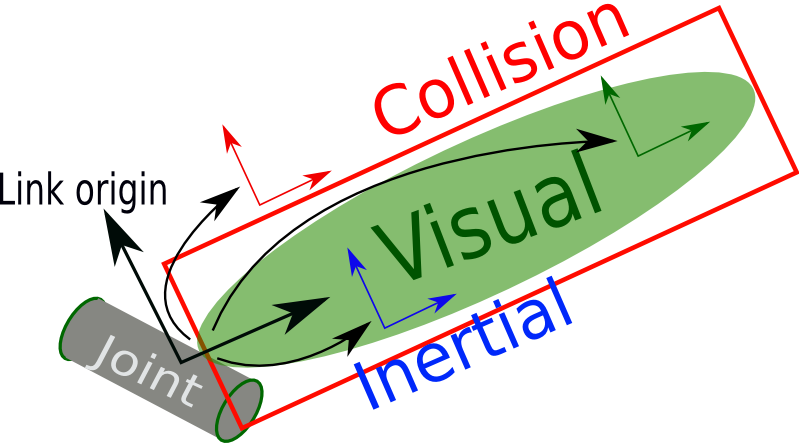
\includegraphics[width=0.60\textwidth]{chapter3/images/urdf_link.png}
	\caption{การอธิบาย link ใน URDF ไฟล์}
	\label{fig:urdf_link}
\end{figure}

\clearpage
\subsubsection*{Joint}
อีกส่วนที่สำคัญสำหรับการสร้างไฟล์หุ่นยนต์ด้วย URDF ก็คือ Joint tag โดย tag นี้จะอธิบายถึงความสัมพันธ์ระหว่างก้านต่อสองอัน
ส่วนนี้ไม่ได้มีเพียงแค่ทำข้อต่อให้เป็นแบบหมุนได้อย่างเดียว ยังมี Fix, Revolution, Linear และ Planar นอกเหนือจากนี้
เรายังสามารถที่จะเพิ่มองศาสูงสุดต่ำสุดของข้อต่อ รวมไปถึง dynamic properties ต่างๆ ตามที่เห็นดังรูปที่ \ref{fig:urdf_joint_code}
\begin{figure}[h!]
\begin{Verbatim}[fontsize=\small]
<joint name="my_joint" type="floating">
	<origin xyz="0 0 1" rpy="0 0 3.1416"/>
	<parent link="link1"/>
	<child link="link2"/>
	<calibration rising="0.0"/>
	<dynamics damping="0.0" friction="0.0"/>
	<limit effort="30" velocity="1.0" lower="-2.2" upper="0.7"/>
	<safety_controller k_velocity="10" k_position="15" 
	soft_lower_limit="-2.0" soft_upper_limit="0.5"/>
</joint>
\end{Verbatim}
\caption{ตัวอย่าง joint ใน urdf}
	\label{fig:urdf_joint_code}
\end{figure}

เมื่อเรานำ Joint และ Link มารวมกันเราจะต้องพิจารณาว่ามีวางรูปแบบเป็นไปตามรูปที่ \ref{fig:urdf_joint}
โดยจะมีระยะระหว่างแกนของแต่ละข้อต่อกับก้านต่อ ชิ้นส่วนแรกของการสร้างไฟล์ URDF จะมีชื่อว่า base\_link
และเฟรม origin จะเป็นเฟรมอ้างอิง เมื่อเราต่อ Joint เข้ากับ Link จะเรียกก้านต่อที่เอามาติดว่า parent
โดยเฟรม origin ของข้อต่อจะอยู่จุดเดียวกับเฟรม origin ของก้านต่อ ในสถานะเดียวกันก้านต่อที่นำมาต่อจากข้อต่อ
เราจะเรียกว่า child และเฟรม origin ของก้านต่อ child จะอยู่ที่จุดเดียวกับเฟรม origin ของข้อต่อ

\begin{figure}[h!]
	\centering
	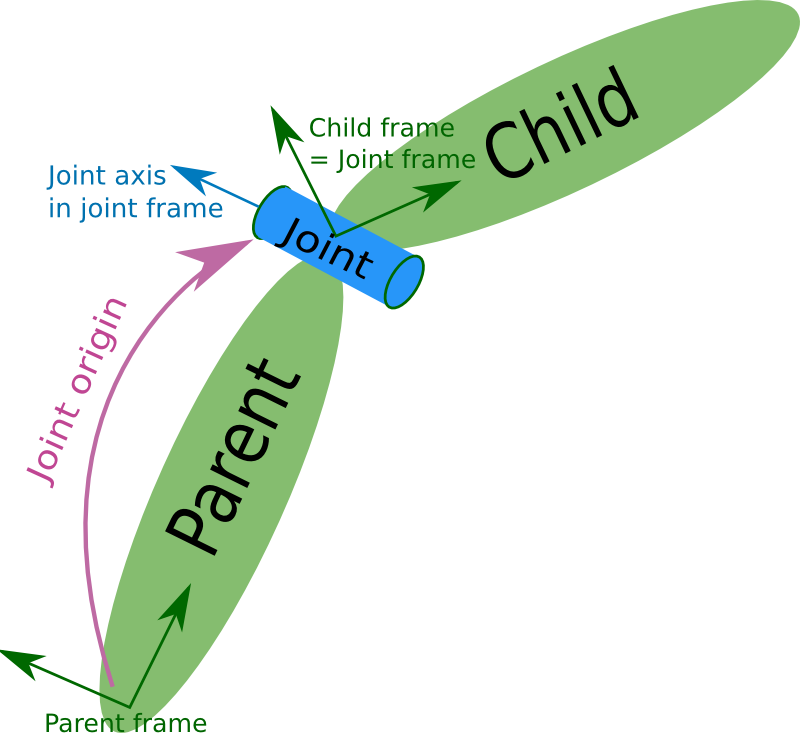
\includegraphics[width=0.55\textwidth]{chapter3/images/urdf_joint.png}
	\caption{การอธิบาย Joint ใน URDF ไฟล์}
	\label{fig:urdf_joint}
\end{figure}

%%%%%%%%%%%%%%%%%%%%%%%%%%%%%%%%%%%%%%%%%%%%%%%%%%%%%%%%%%%%%%%%%%%%%%%%%%%%%%%
\clearpage
\subsection{กำหนดพิกัดเฟรมให้กับหุ่นยนต์ฮิวมานอยด์}
การกำหนดเฟรมให้กับหุ่นยนต์ฮิวมานอยด์นั้นเราจะใช้หลักตามของ ROS Enhancement Proposals (REPs) ซึ่งจะทำให้เราสามารถใช้เครื่องมือต่างๆ ที่มีคนสร้างขึ้นมาใช้งานได้ง่าย และช่วยทำให้เกิดความเข้าใจได้ง่าย

\subsubsection*{base\_link}
เป็นเฟรมที่ติดอยู่กับฐานของหุ่นยนต์ โดยจะติดตำแหน่งหรือมุมเอียงใดก็ได้ ปกติแล้วจะติดที่สะโพกของหุ่นยนต์

\subsubsection*{base\_footprint}
เป็นเฟรมที่เอาไว้แสดงว่าหุ่นยนต์อยู่ตรงไหนบนพื้นโลก โดยปกติแล้วจะมีระดับอยู่ที่จุดต่ำสุดของฝ่าเท้า z = min(l\_sole\_z,r\_sole\_z)
โดย l\_sole\_z และ r\_sole\_z คือความสูงของฝ่าเท้าซ้ายและขวา base\_footprint เหมือน 2D planar
ที่บอกตำแหน่งของฮิวมานอยด์ระหว่างที่กำลังเดินหรือทำอย่างอื่นอยู่

\subsubsection*{l\_wrist, r\_wrist}
เป็นเฟรมที่บอกตำแหน่งและมุมเอียงของแขนซ้ายและขวาแต่ไม่ได้คำนึงถึงการติดตั้งอุปกรณ์ใดๆเข้าไป

\subsubsection*{l\_gripper, r\_gripper}
เป็นเฟรมที่บอกตำแหน่งและมุมเอียงของที่ปลายแขน (End effector) ถ้ามือจับอุปกรณ์อยู่ เฟรมนี้ก็จะไปอยู่ในตำแหน่งของอุปกรณ์นั้นๆ

\subsubsection*{l\_ankle, r\_ankle}
เป็นเฟรมที่บอกตำแหน่งและมุมเอียงของขาซ้ายและขวาโดยไม่ได้คำนึงว่าจุดรับน้ำหนักของตัวอยู่ที่ไหน

\subsubsection*{l\_sole, r\_sole}
เป็นเฟรมที่บอกตำแหน่งและมุมเอียงของขาซ้ายและขวาที่รองรับน้ำหนักตัวอยู่ โดยจะบอกการ projection ของ X,Y ใน 2D plane ที่สัมผัสพื้นและ Z จะอยู่ระดับเดียวกับพื้นสัมผัส

\subsubsection*{l\_toe, r\_toe}
เป็นเฟรมที่บอกตำแหน่งและมุมเอียงของปลายเท้าซ้ายและขวา โดยอยู่บนพื้นผิวที่สัมผัสอยู่

\subsubsection*{gaze}
เป็นเฟรมที่บอกตำแหน่งและมุมเอียงของหัว โดยการเอียงนั้นจะบอกทิศทางของหัวโดยไม่ได้สนใจเซนเซอร์ว่าจะติดตั้งอย่างไร

\subsubsection*{torso}
เป็นเฟรมที่ติดอยู่กับลำตัวช่วงล่างของหุ่นยนต์โดยจะเป็นตัวที่เชื่อม ขา แขน ตัว หัว เข้าเอาไว้ด้วยกัน
%%%%%%%%%%%%%%%%%%%%%%%%%%%%%%%%%%%%%%%%%%%%%%%%%%%%%%%%%%%%%%%%%%%%%%%%%%%%%%%


\clearpage
\subsection{Box model}

\clearpage
\newcommand{\addprop}[9]{
	CoM X (m) & #1\\
	CoM Y (m) & #2\\
	CoM Z (m) & #3\\
	Inertia Ixx & #4\\
	Inertia Ixy & #5\\
	Inertia Ixz & #6\\
	Inertia Iyy & #7\\
	Inertia Iyz & #8\\
	Inertia Izz & #9\\
}

\subsection{Dynamic properties}
ข้อมูลพลศาสตร์ของหุ่นยนต์จะเอาไว้ใช้ในการทำ Simulation บนระบบ ROS และเอาไปใช้ในการคำนวณทางคณิตศาสตร์ได้
โดยข้อมูลนี้เอามาจาก SolidWorks แล้วปรับให้มีค่าใกล้เคียงกับของจริงมากที่สุด

ข้อมูลที่จำเป็นในการใช้งานจะประกอบไปด้วย มวล จุดศูนย์กลางมวล และโมเมนต์ความเฉื่อย

\subsubsection*{Overall Humanoid}
\begin{figure}[!ht]
	\centering
	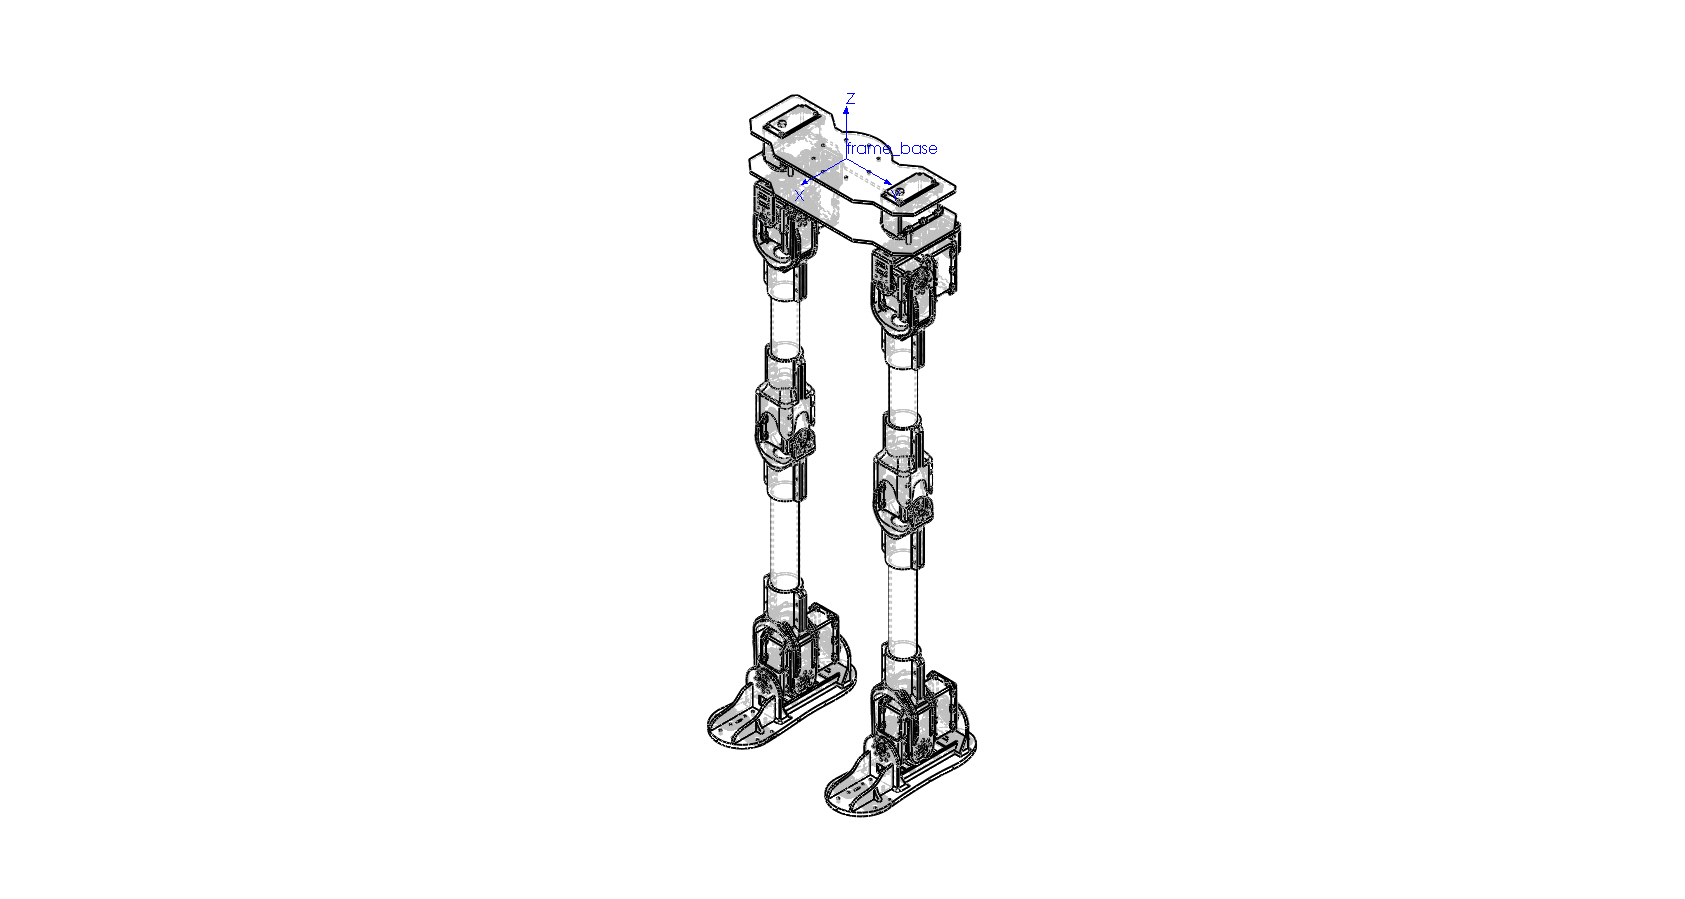
\includegraphics[width=\textwidth]{chapter3/images/uthai_dynamic_all.jpeg}
	\caption{ภาพแสดงช่วงล่างทั้งตัว}
	\label{fig:uthai_dynamic_all}
\end{figure}
\begin{table}[!ht]
	\centering
	\begin{tabular}{| c | c |}
		\hline
		Link & All Link\\
		\hline
		Mass (kg) & 3.31477475 \\
		\addprop{-0.00855772}{0.00000000}{-0.33375492}{0.28641029}{-0.00000302}{-0.00048106}{0.26207601}{-0.00061103}{0.02925799}
		\hline
	\end{tabular}
	\caption{ตารางแสดงค่าพารามิเตอร์ทั้งตัว}
	\label{tab:uthai_dynamic_all}
\end{table}


\newcommand{\adddynamicprop}[6]{
	\clearpage
	\subsubsection*{#1}
	\begin{figure}[!ht]
		\centering
		\includegraphics[width=\textwidth]{chapter3/images/{#2}.jpeg}
		\caption{ภาพแสดงก้านต่อ #1}
	\end{figure}
	\begin{table}[!ht]
		\begin{subtable}[b]{0.45\textwidth}
			\centering
			\begin{tabular}{| c | c |}
				\hline
				Link & #3\\
				\hline
				Mass (kg) & #4\\
				\addprop#5
				\hline
			\end{tabular}
			\caption{DH Parameter}
		\end{subtable}
		\begin{subtable}[b]{0.45\textwidth}
			\centering
			\begin{tabular}{| c | c |}
				\hline
				Link & #3\\
				\hline
				Mass (kg) & #4\\
				\addprop#6
				\hline
			\end{tabular}
			\caption{URDF}
		\end{subtable}
		\caption{ตารางแสดงค่าพารามิเตอร์ #1}
	\end{table}
	}
%{header name}{file name}{link name}{mass}
%{{comXdh}{comYdh}{comZdh}{Ixxdh}{Ixydh}{Ixzdh}{Iyydh}{Iyzdh}{Izzdh}}
%{{comXurdf}{comYurdf}{comZurdf}{Ixxurdf}{Ixyurdf}{Ixzurdf}{Iyyurdf}{Iyzurdf}{Izzurdf}}

\adddynamicprop{Right Hip Yaw}{uthai_dynamic_rhy}{r\_hip\_yaw}{0.09100000}
{{0.00000000}{0.02864983}{-0.02500000}{0.00014158}{0.00000000}{0.00000000}{0.00014316}{0.00000000}{0.00002022}}
{{0.00000000}{-0.02500000}{-0.00735017}{0.00014158}{0.00000000}{0.00000000}{0.00002022}{0.00000000}{0.00014316}}

\adddynamicprop{Left Hip Yaw}{uthai_dynamic_lhy}{l\_hip\_yaw}{0.09100000}
{{0.00000000}{0.02864983}{-0.02500000}{0.00014158}{0.00000000}{0.00000000}{0.00014316}{0.00000000}{0.00002022}}
{{0.00000000}{0.02500000}{-0.00735017}{0.00014158}{0.00000000}{0.00000000}{0.00002022}{0.00000000}{0.00014316}}

\adddynamicprop{Right Hip Roll}{uthai_dynamic_rhr}{r\_hip\_roll}{0.34300000}
{{0.01526237}{0.02152630}{0.00000000}{0.00026846}{0.00000219}{-0.00000081}{0.00014760}{0.00000000}{0.00032448}}
{{0.00000000}{-0.01526237}{-0.02652630}{0.00032448}{0.00000081}{0.00000000}{0.00026846}{0.00000219}{0.00014760}}

\adddynamicprop{Left Hip Roll}{uthai_dynamic_lhr}{l\_hip\_roll}{0.34300000}
{{0.01526237}{0.02152630}{0.00000000}{0.00026846}{0.00000219}{-0.00000081}{0.00014760}{0.00000000}{0.00032448}}
{{0.00000000}{-0.01526237}{-0.02652630}{0.00032448}{0.00000081}{0.00000000}{0.00026846}{0.00000219}{0.00014760}}

\adddynamicprop{Right Hip Pitch}{uthai_dynamic_rhp}{r\_hip\_pitch}{0.31800000}
{{-0.07862011}{0.00000000}{0.00000000}{0.00011525}{0.00000000}{0.00000078}{0.00254669}{0.00000000}{0.00250848}}
{{0.22137989}{0.00000000}{0.00000000}{0.00011525}{0.00000000}{0.00000078}{0.00254669}{0.00000000}{0.00250848}}

\adddynamicprop{Left Hip Pitch}{uthai_dynamic_lhp}{l\_hip\_pitch}{0.31800000}
{{-0.07862011}{0.00000000}{0.00000000}{0.00011525}{0.00000000}{0.00000078}{0.00254669}{0.00000000}{0.00250848}}
{{0.22137989}{0.00000000}{0.00000000}{0.00011525}{0.00000000}{0.00000078}{0.00254669}{0.00000000}{0.00250848}}

\adddynamicprop{Right Knee Pitch}{uthai_dynamic_rkp}{r\_knee\_pitch}{0.13800000}
{{-0.15211782}{0.00000000}{0.00000000}{0.00011525}{0.00000000}{0.00000000}{0.00127592}{0.00000000}{0.00124960}}
{{0.16288218}{0.00000000}{0.00000000}{0.00005794}{0.00000000}{0.00000000}{0.00127592}{0.00000000}{0.00124960}}

\adddynamicprop{Left Knee Pitch}{uthai_dynamic_lkp}{l\_knee\_pitch}{0.13800000}
{{-0.15211782}{0.00000000}{0.00000000}{0.00011525}{0.00000000}{0.00000000}{0.00127592}{0.00000000}{0.00124960}}
{{0.16288218}{0.00000000}{0.00000000}{0.00005794}{0.00000000}{0.00000000}{0.00127592}{0.00000000}{0.00124960}}

\adddynamicprop{Right Ankle Pitch}{uthai_dynamic_rap}{r\_ankle\_pitch}{0.33138738}
{{-0.01526237}{0.00000000}{-0.02152630}{0.00025937}{0.00000000}{0.00000079}{0.00031349}{0.00000000}{0.00014261}}
{{-0.01526237}{0.02152630}{0.00000000}{0.00025937}{0-0.00000212}{0.00000079}{0.00014261}{0.00000000}{0.00031349}}

\adddynamicprop{Left Ankle Pitch}{uthai_dynamic_lap}{l\_ankle\_pitch}{0.33138738}
{{-0.01526237}{0.00000000}{-0.02152630}{0.00025937}{0.00000000}{0.00000079}{0.00031349}{0.00000000}{0.00014261}}
{{-0.01526237}{0.02152630}{0.00000000}{0.00025937}{0-0.00000212}{0.00000079}{0.00014261}{0.00000000}{0.00031349}}

\adddynamicprop{Right Ankle Roll}{uthai_dynamic_rar}{r\_ankle\_roll}{0.10500000}
{{-0.01454118}{-0.00034576}{-0.00019548}{0.00034591}{-0.00000857}{-0.00000013}{0.00004813}{-0.00000120}{0.00032705}}
{{0.03625882}{-0.00019548}{0.00034576}{0.00034591}{-0.00000013}{0.00000857}{0.00032705}{0.00000120}{0.00004813}}

\adddynamicprop{Left Ankle Roll}{uthai_dynamic_lar}{l\_ankle\_roll}{0.10500000}
{{-0.01454118}{-0.00034576}{-0.00019548}{0.00034591}{-0.00000857}{-0.00000013}{0.00004813}{-0.00000120}{0.00032705}}
{{0.03625882}{-0.00019548}{0.00034576}{0.00034591}{-0.00000013}{0.00000857}{0.00032705}{0.00000120}{0.00004813}}

%%%%%%%%%%%%%%%%%%%%%%%%%%%%%%%%%%%%%%%%%%%%%%%%%%%%%%%%%%%%%%%%%%%%%%%%%%%%%%%
%%%%%%%%%%%%%%%%%%%%%%%%%%%%%%%%%%%%%%%%%%%%%%%%%%%%%%%%%%%%%%%%%%%%%%%%%%%%%%%
\clearpage
\subsection{โครงสร้างการติดต่อสื่อสารระหว่าง Node ใน ROS}
การติดต่อสื่อสารกันภายใน ROS นั้นจะใช้การส่ง message หากัน ซึ่ง message แต่ละตัวก็จะใช้ในงานที่ต่างกัน
ตามระบบที่ต้องการส่ง จากรูปที่ \ref{fig:uthai_ros_node} เป็นโครงสร้างการส่งข้อมูลหากันของหุ่นยนต์ฮิวมานอยด์
ที่ผู้วิจัยได้ออกแบบไว้ โดยเริ่มจากผู้ใช้งานส่งตำแหน่งที่หุ่นยนต์จะต้องเดินไปไปยัง Node ที่ทำการคำนวณและสร้างตำแหน่งการวางเท้าของหุ่นยนต์
แล้วหลังจากนั้นจะส่งข้อมูลออกไปเป็น Path เส้นทางไปยัง Node ที่ทำการค้นหาตำแหน่งของ com, zmp ของหุ่นยนต์
เพื่อทำการควบคุมและสั่งการหุ่นยนต์ต่อไป

\begin{figure}[h!]
	\centering
	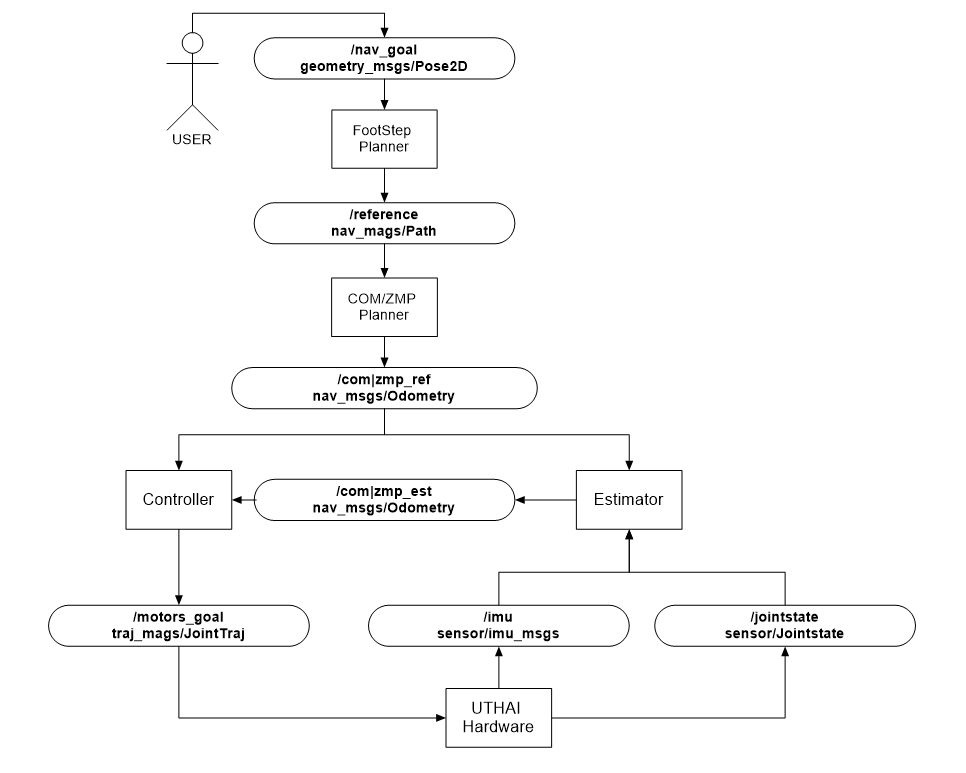
\includegraphics[width=\textwidth]{chapter3/images/uthai_ros_node.png}
	\caption{การติดต่อสื่อสารระหว่าง Node}
	\label{fig:uthai_ros_node}
\end{figure}

\subsubsection*{การบอกตำแหน่งและมุมเอียง}
การบอกตำแหน่งใน 3 มิติ Point คือการบอก $x$, $y$, $z$ และการบอกมุมเอียงจะใช้ Quaternion
ในการบอกโดยใช้ตัวแปรสี่ตัว คือ $x$,$y$,$z$,$w$ หากนำทั้งสองมารวมกันเราจะเรียกว่า Pose
\begin{table}[h!]
	\centering
	\begin{tabular}{| c | c |}
		\hline
		\multicolumn{2}{|c|}{geometry\_msgs/Point}\\
		\hline
		float64 & x \\
		float64 & y \\
		float64 & z \\
		\hline
	\end{tabular}
	\caption{Message Geometry Point}
	\label{tab:geometry_point}
\end{table}
\begin{table}[h!]
	\centering
	\begin{tabular}{| c | c |}
		\hline
		\multicolumn{2}{|c|}{geometry\_msgs/Quaternion}\\
		\hline
		float64 & x \\
		float64 & y \\
		float64 & z \\
		float64 & w \\
		\hline
	\end{tabular}
	\caption{Message Geometry Quaternion}
	\label{tab:geometry_quaternion}
\end{table}
\begin{table}[h!]
	\centering
	\begin{tabular}{| c | c |}
		\hline
		\multicolumn{2}{|c|}{geometry\_msgs/Pose}\\
		\hline
		geometry\_msgs/Point & position \\
		geometry\_msgs/Quaternion & orientation \\
		\hline
	\end{tabular}
	\caption{Message Geometry Pose}
	\label{tab:geometry_pose}
\end{table}

\subsubsection*{การบอกความเร็วเชิงเส้นและเชิงมุม}
การบอกความเร็วเชิงเส้นใน 3 มิติ คือการบอกความเร็วตามแนวแกน $x$, $y$, $z$ และการบอกความเร็วเชิงมุม
คือการบอกความเร็วการหมุนรอบแกน $x$,$y$,$z$ หากนำทั้งสองมารวมกันเราจะเรียกว่า Twist
\begin{table}[h!]
	\centering
	\begin{tabular}{| c | c |}
		\hline
		\multicolumn{2}{|c|}{geometry\_msgs/Vector3}\\
		\hline
		float64 & x \\
		float64 & y \\
		float64 & z \\
		\hline
	\end{tabular}
	\caption{Message Geometry Vector3}
	\label{tab:geometry_vector3}
\end{table}
\begin{table}[h!]
	\centering
	\begin{tabular}{| c | c |}
		\hline
		\multicolumn{2}{|c|}{geometry\_msgs/Twist}\\
		\hline
		geometry\_msgs/Vector3 & linear \\
		geometry\_msgs/Vector3 & angular \\
		\hline
	\end{tabular}
	\caption{Message Geometry Twist}
	\label{tab:geometry_twist}
\end{table}

\subsubsection*{การบอกตำแหน่งและความเร็ว}
หากนำทั้งสองมารวมกันระกว่าง ตำแหน่ง(Pose) และความเร็ว (Twist) เราจะเรียกว่า Odometry
แต่ที่เพิ่มเข้ามาคือ Covariance ซึ่งอาจทำให้เกิดความสับสนได้
\begin{table}[h!]
	\centering
	\begin{tabular}{| c | c |}
		\hline
		\multicolumn{2}{|c|}{nav\_msgs/Odometry}\\
		\hline
		std\_msgs/Header & header \\
		geometry\_msgs/PoseWithCovariance & pose \\
		geometry\_msgs/TwistWithCovariance & twist \\
		\hline
	\end{tabular}
	\caption{Message Navigation Odometry}
	\label{tab:nav_odometry}
\end{table}

\clearpage
\subsubsection*{ตำแหน่งของหุ่นยนต์}
การบอกตำแหน่งของหุ่นยนต์บนระนาบ 2 มิติ คือการบอก $x$, $y$ และ $\theta$
การบอกนั้นจะบอกว่าตำแหน่งที่หุ่นยนต์อยู่นั้นอยู่ตรงไหนหากเที่ยบกับแผนที่
รวมไปถึงตำแหน่งของหุ่นยนต์ที่ต้องการจะเดินไปด้วย ซึ่งอ้างอิงมาจากตำแหน่งเริ่มต้นของแผนที่ 
\begin{table}[h!]
	\centering
	\begin{tabular}{| c | c |}
		\hline
		\multicolumn{2}{|c|}{geometry\_msgs/Pose2D}\\
		\hline
		float64 & x \\
		float64 & y \\
		float64 & theta \\
		\hline
	\end{tabular}
	\caption{Message Geometry Pose2D}
	\label{tab:geometry_pose2d}
\end{table}

\subsubsection*{ตำแหน่งการวางเท้าของหุ่นยนต์}
การจะให้หุ่นยนต์นำเท้าไปวางในตำแหน่งที่เราต้องการจากที่ได้จากการคำนวณนั้น
จะต้องบอกตำแหน่งและบอกมุมเอียงของจุดที่จะไป จากการสร้างจะได้เป็นรายการของเท้าซ้ายและขวา
โดยอิงจาก ตารางที่ \ref{tab:geometry_pose}
\begin{table}[h!]
	\centering
	\begin{tabular}{| c | c |}
		\hline
		\multicolumn{2}{|c|}{nav\_msgs/Path}\\
		\hline
		std\_msgs/Header & header \\
		geometry\_msgs/PoseStamped[] & poses \\
		\hline
	\end{tabular}
	\caption{Message Navigation Path}
	\label{tab:nav_path}
\end{table}
\begin{table}[h!]
	\centering
	\begin{tabular}{| c | c |}
		\hline
		\multicolumn{2}{|c|}{geometry\_msgs/PoseStamped}\\
		\hline
		std\_msgs/Header & header \\
		geometry\_msgs/Pose & pose \\
		\hline
	\end{tabular}
	\caption{Message Geometry PoseStamped}
	\label{tab:geometry_posestamped}
\end{table}

\subsubsection*{ตำแหน่ง CoM Zmp ของหุ่นยนต์}
ใน Message นี้จะใช้อยู่ 2 จุดคือ ที่ได้จากการวางแผนของ Node CoM Planner และ Node CoM Estimator
โดยทั้งสองจุดใช้ Message เหมือนกันส่งไปยัง Controller เพื่อควบคุมท่าทางต่างๆของหุ่นยนต์ต่อไป
Message ที่ใช้คือ Message จากตารางที่ \ref{tab:nav_odometry}
\begin{table}[h!]
	\centering
	\begin{tabular}{| c | c |}
		\hline
		\multicolumn{2}{|c|}{nav\_msgs/Odometry}\\
		\hline
		std\_msgs/Header & header \\
		geometry\_msgs/PoseWithCovariance & pose \\
		geometry\_msgs/TwistWithCovariance & twist \\
		\hline
	\end{tabular}
	\caption*{Message Navigation Odometry}
\end{table}

\clearpage
\subsubsection*{การควบคุมข้อต่อของหุ่นยนต์}
ในการควบคุมข้อต่อแต่ละข้อของหุ่นยนต์ฮิวมานอยด์นั้นจะใช้ Message trjectory\_msgs/JointTrajectory
ซึ่งสามารถส่ง ตำแหน่ง ความเร็ว ความเร่ง และ แรงบิด ไปได้ ทำให้หากต้องการเปลี่ยนระบบใหม่สามารถทำได้โดยง่าย

\begin{table}[h!]
	\centering
	\begin{tabular}{| c | c |}
		\hline
		\multicolumn{2}{|c|}{trajectory\_msgs/JointTrajectory}\\
		\hline
		std\_msgs/Header & header \\
		string[] & joint\_names \\
		trajectory\_msgs\_msgs/JointTrajectoryPoint[] & points \\
		\hline
	\end{tabular}
	\caption{Message Trajectory JointTrajectory}
	\label{tab:trajectory_jointrajectory}
\end{table}
\begin{table}[h!]
	\centering
	\begin{tabular}{| c | c |}
		\hline
		\multicolumn{2}{|c|}{trajectory\_msgs/JointTrajectoryPoint}\\
		\hline
		float64[] & positions \\
		float64[] & velocities \\
  		float64[] & accelerations \\
  		float64[] & effort \\
  		duration & time\_from\_start \\
		\hline
	\end{tabular}
	\caption{Message Trajectory JointTrajectoryPoint}
	\label{tab:trajectory_jointrajectorypoint}
\end{table}

\subsubsection*{ค่าเซนเซอร์ข้อต่อของหุ่นยนต์}
ที่ข้อต่อของหุ่นยนต์ฮิวมานอยด์มีเซนเซอรที่เอาไว้ใช้ในการอ่านค่าตำแหน่ง ความเร็ว และแรง อยู่ด้วย
เราสามารถที่จะใช้ Message sensor\_msgs/JointState สำหรับอ่านค่าตำแหน่ง ความเร็ว แรง
ของตัวขับเคลื่อนแล้วส่งให้ Estimater Node ได้
\begin{table}[h!]
	\centering
	\begin{tabular}{| c | c |}
		\hline
		\multicolumn{2}{|c|}{sensor\_msgs/JointState}\\
		\hline
		std\_msgs/Header & header \\
		float64[] & position \\
		float64[] & velocity \\
		float64[] & effort \\
		\hline
	\end{tabular}
	\caption{Message Sensor JointState}
	\label{tab:sensor_jointstate}
\end{table}

\subsubsection*{ค่าเซนเซอร์ฝ่าเท้าของหุ่นยนต์}
ที่ฝ่าเท้าของหุ่นยนต์ฮิวมานอยด์มีเซนเซอรที่เอาไว้ใช้ในการอ่าน แรงกดที่ฝ่าเท้า ใช้ในการเอามาบอกว่าเท้าสัมผัสพื้นหรือไม่
\begin{table}[h!]
	\centering
	\begin{tabular}{| c | c |}
		\hline
		\multicolumn{2}{|c|}{geometry\_msgs/Wrench}\\
		\hline
		geometry\_msgs/Vector3 & force \\
		geometry\_msgs/Vector3 & torque \\
		\hline
	\end{tabular}
	\caption{Message Geometry Wrench}
	\label{tab:geometry_wrench}
\end{table}

\clearpage
\subsubsection*{ค่าเซนเซอร์ IMU ของหุ่นยนต์}
เซนเซอร์ IMU เป็นเซนเซอร์ที่เอาไว้ใช้ในการวัด ความเร็วเชิงมุม และ ความเร่งเชิงเส้น
หากนำทั้งคู่มารวมกันจะสามารถที่จะแปลงให้วัดมุมเอียงของเซนเซอร์ได้ โดยจะใช้ Message
std\_msgs/Imu ในการส่งให้ Node Estimator จากตัวหุ่นยนต์
\begin{table}[h!]
	\centering
	\begin{tabular}{| c | c |}
		\hline
		\multicolumn{2}{|c|}{sensor\_msgs/Imu}\\
		\hline
		std\_msgs/Header & header \\
		geometry\_msgs/Quaternion & orientation \\
		float64[9] & orientation\_covariance \\
		geometry\_msgs/Vector3 & angular\_velocity \\
		float64[9] & angular\_velocity\_covariance \\
		geometry\_msgs/Vector3 & linear\_acceleration \\
		float64[9] & linear\_acceleration\_covariance \\
		\hline
	\end{tabular}
	\caption{Message Sensor Imu}
	\label{tab:sensor_imu}
\end{table}
\begin{table}[h!]
	\centering
	\begin{tabular}{| c | c |}
		\hline
		\multicolumn{2}{|c|}{sensor\_msgs/MegneticField}\\
		\hline
		std\_msgs/Header & header \\
		geometry\_msgs/Vector3 & magnetic\_field \\
		float64[9] & magnetic\_field\_covariance \\
		\hline
	\end{tabular}
	\caption{Message Sensor MegneticField}
	\label{tab:sensor_megneticfield}
\end{table}
%%%%%%%%%%%%%%%%%%%%%%%%%%%%%%%%%%%%%%%%%%%%%%%%%%%%%%%%%%%%%%%%%%%%%%%%%%%%%%%
%%%%%%%%%%%%%%%%%%%%%%%%%%%%%%%%%%%%%%%%%%%%%%%%%%%%%%%%%%%%%%%%%%%%%%%%%%%%%%%